\documentclass{beamer}

\usecolortheme[light]{solarized}

\beamertemplatenavigationsymbolsempty

\usepackage{hyperref}
\usepackage{minted}

\usepackage{graphicx}
\usepackage{tikz}

\usetikzlibrary{calc, patterns}

\begin{document}

    \begin{frame}
        \begin{center}
            \Large

            ``I will not lecture you.''

            \normalsize
            \vspace{1cm}
            Vince\\
            \href{https://twitter.com/drvinceknight}{@drvinceknight}\\
            \texttt{knightva@cardiff.ac.uk}
        \end{center}


    \end{frame}

    \begin{frame}
        \begin{center}
            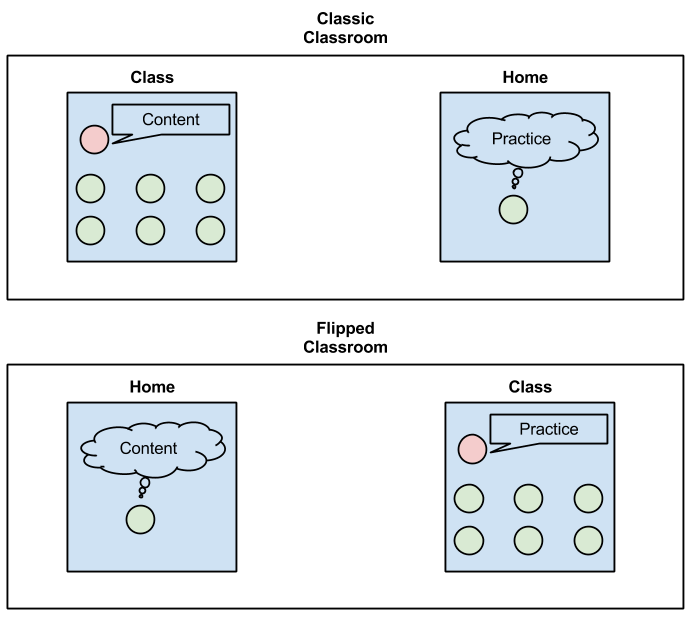
\includegraphics[width=.8\textwidth]{./static/flipped_class.png}
        \end{center}
    \end{frame}

    \begin{frame}
		\begin{center}
			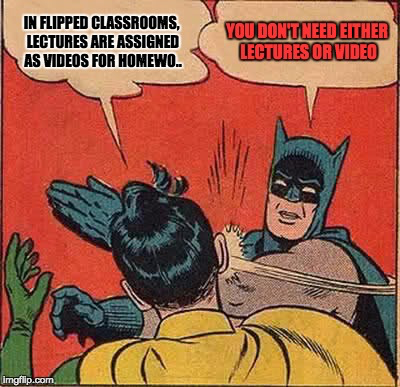
\includegraphics[width=.6\textwidth]{./static/time_for_this_again.png}
		\end{center}
	\end{frame}

    \begin{frame}
        \Huge
        \begin{center}
			Initial contact.
        \end{center}
    \end{frame}

    \begin{frame}
		\begin{center}
            \frame{
\includegraphics[height=.8\textheight]{./static/flipped_learning.jpg}}
		\end{center}
	\end{frame}
    \begin{frame}
        \begin{center}
			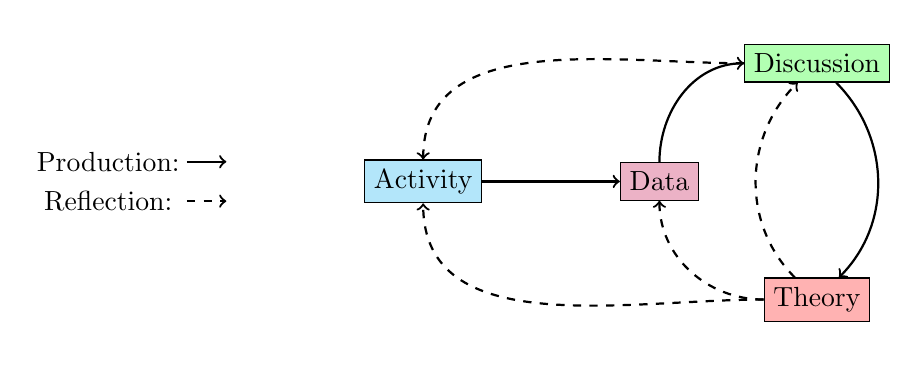
\begin{tikzpicture}
				% Nodes
				\node (activity) at (0,0) [fill=cyan!30, draw] {Activity};
				\node (data) at ($(activity) + (3,0)$) [fill=purple!30, draw] {Data};
				\node (discussion) at ($(data) + (2,1.5)$) [fill=green!30, draw] {Discussion};
				\node (theory) at ($(data) + (2,-1.5)$) [fill=red!30, draw] {Theory};

				% Creative arrows
				\draw [thick, ->] (activity) -- (data);
				\draw [thick, ->] (data) edge[out=90, in=180] (discussion);
				\draw [thick, ->] (discussion) edge[out=-45, in=45] (theory);

				% Reflective arrows
				\draw [thick, ->, dashed] (theory) edge[out=180, in=-90] (data);
				\draw [thick, ->, dashed] (theory) edge[out=180, in=-90] (activity);
				\draw [thick, ->, dashed] (discussion) edge[out=180, in=90] (activity);
				\draw [thick, ->, dashed] (theory) edge[out=135, in=-135] (discussion);

				% Key
				\draw [thick, ->] ($(activity) + (-3,.25)$) -- ($(activity) + (-2.5,.25)$);
				\node at ($(activity) + (-4, .25)$) {Production:};
				\draw [thick, ->, dashed] ($(activity) + (-3,-.25)$) -- ($(activity) +
				(-2.5,-.25)$);
				\node at ($(activity) + (-4, -.25)$) {Reflection:};

			\end{tikzpicture}
        \end{center}

        \begin{center}
            \textbf{Playing Games: A Case Study in Active Learning Applied to Game Theory} Knight. 2015 (MSOR Connections)
        \end{center}
	\end{frame}

    \begin{frame}
            \textbf{FAQ:} Yes, great but [subject] is different.

            \textbf{FAQ:} If I record my class will students no longer attend?

			\textbf{FAQ:} If students don't [do some activity] before class what
            should I do?

            \textbf{FAQ:} I have seen [a good talk] on flipped learning, isn't
            that ironic?

			\textbf{FAQ:} I tried the flipped classroom and students don't like it.

			\textbf{FAQ:} How much more work is it?

			\textbf{FAQ:} Why use this new thing? What we've done before is
            fine.
	\end{frame}

    \begin{frame}
        \begin{center}
            \Large
            Reaction.
        \end{center}
    \end{frame}

    \begin{frame}
        \begin{center}
            \normalsize
            Vince: \href{https://twitter.com/drvinceknight}{@drvinceknight}
            \texttt{knightva@cardiff.ac.uk}
        \end{center}
    \end{frame}

\end{document}
